\subsection{Convolutional Neural Network}
\label{section:BT:CNN}
A \textbf{Convolutional Neural Network (CNN)} is a neural network architecture built using convolutional layers in order to extract information.
Unlike fully connected neural networks, convolutional layers interpret data using perceptive fields.
These perceptive fields evaluate only sections of the input at a time until the whole input is processed.
The convolutional layers attempt to extract features from the input data.
The first layer extracts low-level features, while the next layer extracts higher-level features, and so on
\cite[p.~443-446]{Geron2017}.




\begin{figure}[h!]
  \centering
  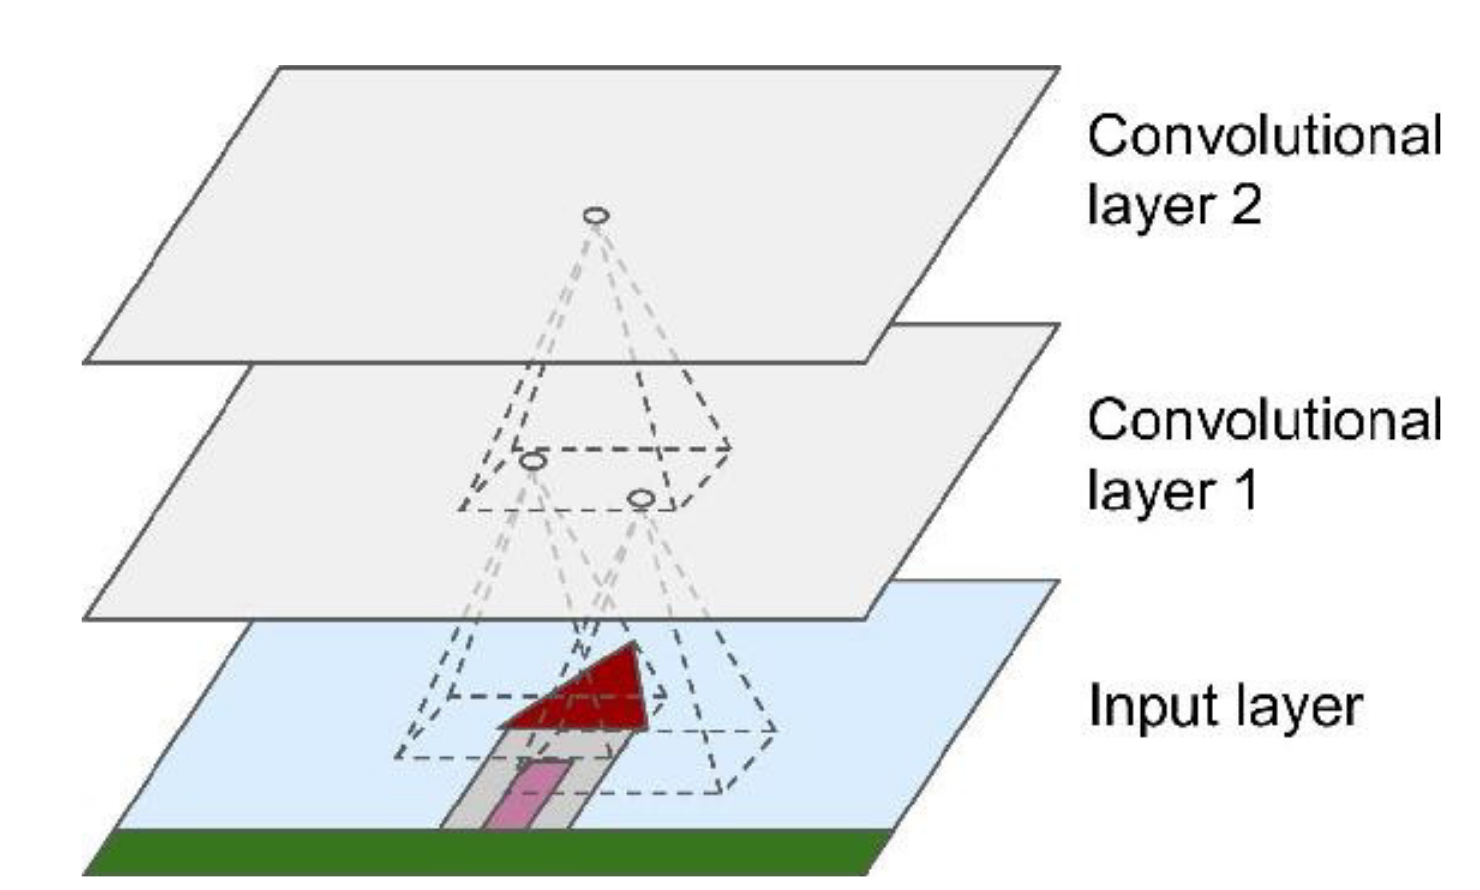
\includegraphics[width=0.7\textwidth]{./sections/BT/figures/convolution_hands_one_machine_learning.png}
  \hfill
  \caption{Figure of CNN layers from \cite[p.~444]{Geron2017}.}
  \label{fig:convolution}
\end{figure}


Multiple kernels, or filters, are used to extract features from the data.
The result of applying these filters is known as the feature map or the extracted data features.
These feature maps extract lower and higher lever features from the original data by
extracting spatial features, retaining the spatial relationship within the data.
Such spatial features could be the curvature of a dog's ears in an image or the correlation of timestep data in a time-series.
As a result, convolutional networks have several applications within image classification,
image recognition, natural language processing, and time-series analysis.



% [Se kilder wikipedia? Eller bare bruke Boka? Dobbelt sjekke]